\chapter{Dataset}
\label{chap:dataset}
	\textit{\hspace{0.5cm}In this chapter, we want to describe the datasets which we use to train and evaluate the Logistic Regression module and CNN categorize module, with the problems of datasets and pre-processing details.}
\minitoc
\section{Logistic regression dataset}
\label{sec:logistic_dataset}
\subsection{CSIC 2010 dataset}
\label{subsec:csic_2010}
\hspace{0.5cm}The HTTP dataset CSIC 2010\footnote{Available at \url{https://www.isi.csic.es/dataset/}} contains web requests automatically generated, both normal and abnormal. It can be used for the testing of web attack protection systems. It was developed at the ``Information Security Institute'' of CSIC (Spanish Research National Council). The HTTP dataset CSIC 2010\index{CSIC 2010} contains the generated traffic targeted to an e-commerce web application developed at their department. In this web application, users can buy items using a shopping cart and register by providing some personal information. As it is a web application in Spanish, the data set contains some Latin characters. A request from the dataset is presented in the following figure (Figure 6.1).

\begin{figure}[ht]
	\centering
	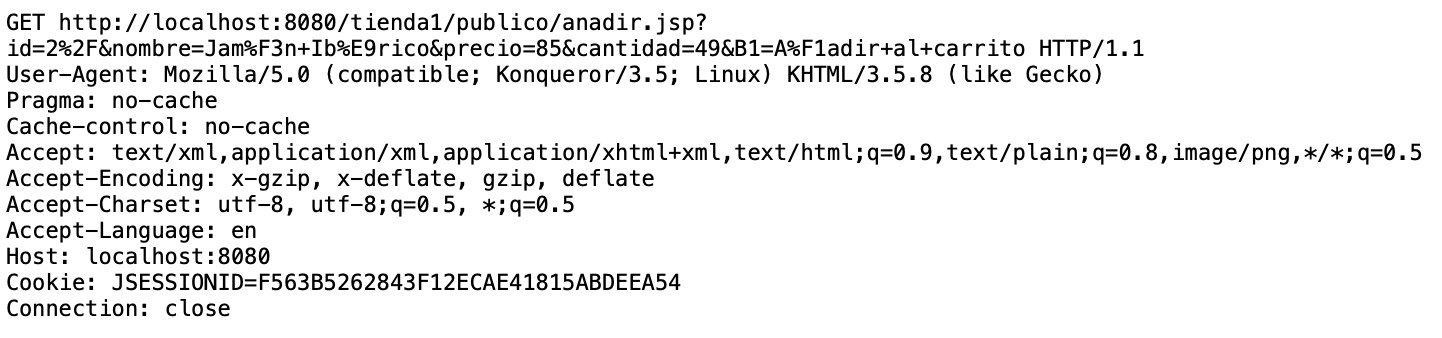
\includegraphics[width=\linewidth, height=10cm,keepaspectratio]{figures/dataset1.png}
  \caption{A sample request of the dataset}
\end{figure} 

The dataset consists of 36,000 legitimate requests and 25,063 anomalous requests. The HTTP requests are labeled as normal or abnormal; the dataset includes attacks such as SQL injection\index{SQLi}, buffer overflow, information gathering, file disclosure, CRLF injection, XSS\index{XSS}, server-side includes injection, parameter tampering, and so on. 

According to the authors, the dataset is generated using the following steps.

1.	Real-life data are collected for all the parameters of the web application. All the data (names, surnames, addresses, etc.) are extracted from actual databases. These values are stored in two databases: one for the normal values and the other for the anomalous ones. Additionally, all the publicly available pages of the web application are listed. 

2.	For every web page, both normal and unusual requests are generated. When standard requests contain parameters, data randomly selected from the standard database is used to fill out the parameter values. The procedure is similar to anomalous requests in which the parameters' values are pulled from the anomalous database.  

In this dataset, three types of anomalous requests were considered. 
\begin{itemize}
	\item Static attacks try to request hidden (or non-existent) resources. These requests include obsolete files, configuration files, default files, etc. 
	\item Dynamic attacks modify valid request arguments: SQLi\index{SQLi}, CRLF injection, XSS\index{XSS}, buffer overflow, etc.
	\item Unintentional illegal requests. These requests do not have malicious intentions, however, they do not follow the normal behavior of the web application and do not have the same structure as normal parameter values.
\end{itemize}

This dataset is quite outdated and randomly generated. It comprises a complete HTTP request with various components such as request URL, request method, pragma, and so on. During our research, we observed that the majority of the indicators of a malicious request may be located in the URL portion of the request. For example, an SQLi\index{SQLi} will have a route that includes a string such as: \textit{2\&nombre=Jam\%F3n+Ib\%E9rico\&precio=85 \\ \&cantidad=\%27\%3B+  DROP +TABLE+usuarios\%3B+SELECT+*+FROM+datos+ \\ WHERE+nombre+LIKE+\%27\%25\&B1=A\%F1adir+al+carrito}.

Consequently, we will solely concentrate on the URL and Method parts of each HTTP request in order to detect fraudulent requests.

\begin{figure}[ht]
	\centering
	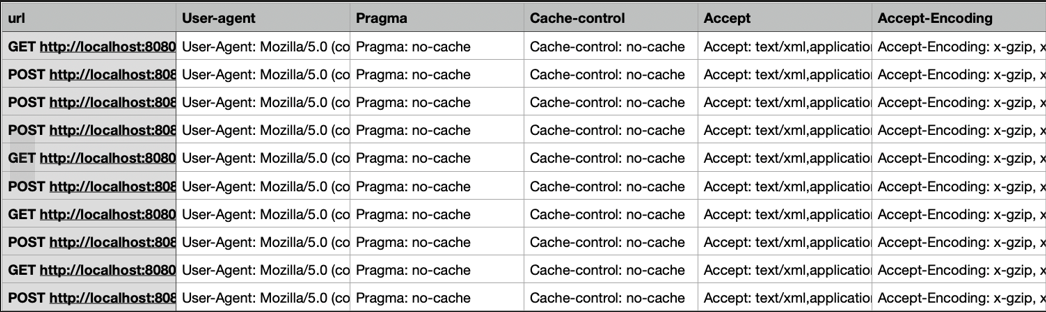
\includegraphics[width=\linewidth, height=10cm,keepaspectratio]{figures/dataset part1.PNG}
	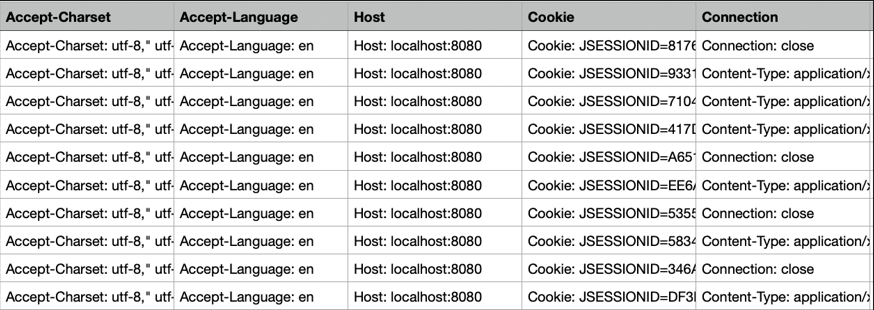
\includegraphics[width=\linewidth, height=10cm,keepaspectratio]{figures/dataset part2.PNG}
  \caption{Requests dataset}
\end{figure}

\newpage
\subsection{Malicious and non-malicious URL}

\hspace{0.5cm}We opted to utilize this extra dataset from Kaggle, with an extremely basic structure, because using only data from the CSIC 2010\index{CSIC 2010} set is not dependable enough for our model to have a high level of reliability. Include just URLs and their labels. It consists of over 400,000 unique already labeled URLs.
\begin{figure}[ht]
	\centering
	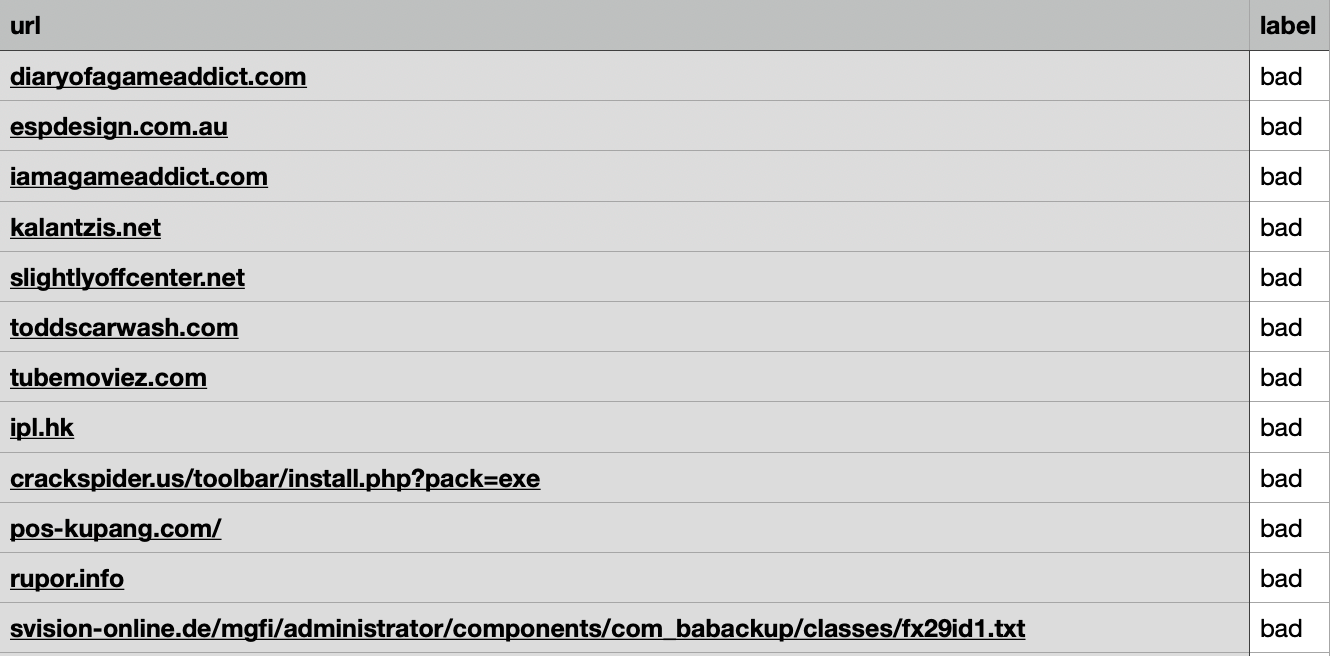
\includegraphics[width=\linewidth, height=10cm,keepaspectratio]{figures/dataset3.png}
  \caption{A set of labeled URLs}
\end{figure}

Another thing to mention is the requests datasets generally are confidential, as they may contain sensitive data of users. There are not many open datasets available. Also, labeling these datasets are costly task, as it requires expertise in the field.

\begin{figure}[ht]
	\centering
	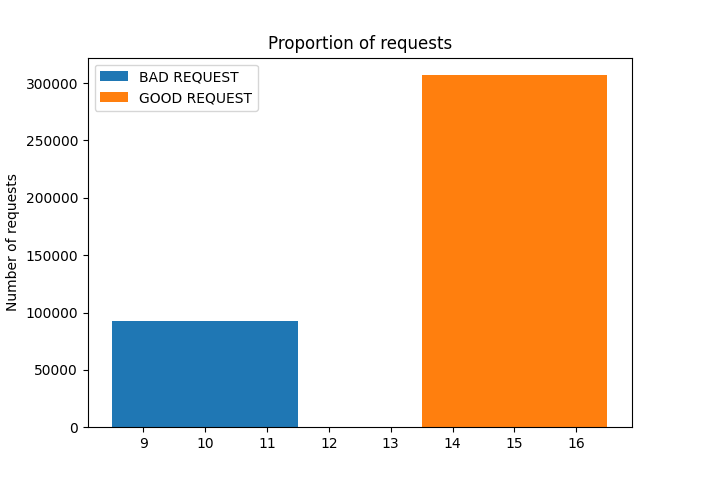
\includegraphics[width=\linewidth, height=8cm,keepaspectratio]{figures/proportion.png} 
  \caption{Proportion of requests}
\end{figure}


\newpage
\section{CNN classification module}
\label{sec:CNN_module}
\hspace{0.5cm}The malicious request validator module detects the category of requests. As the categories are mostly structured languages (four out of five categories), we need to get a dataset of structured language and its category, as proposed in the proposed approach.

This dataset contains over 97,000,000 snippets of code from various GitHub repositories with more than 10,000 stars. The repositories included in this dataset were the results of searching for repositories with greater than 10,000 stars. For each repository, we created snippets from the default branch by going through each text file and extracting 5-line chunks of text every 5 lines. The dataset used file extensions to associate snippets with the programming language they most likely represent. For snippets for which it could not infer the language from the file extension, it uses the value UNKNOWN in the language column.

This dataset is very large, stored in an SQLite database, and includes many languages, so data preprocessing is very critical. We use a Python script to extract randomly 400,000 snippets of code from the database, and only from the languages relevant to our classification in the proposed approach.

The list consist of these categories.
\begin{itemize}
	\item Plain text: JSON, HTML, YAML
	\item Client-side script: JavaScript
	\item Server-side script: PhP, Go, Python, C, C++
	\item Shell script: Shell
	\item SQL script: SQL 
\end{itemize}

The shorten dataset is presented in Figure 6.5.

\begin{figure}[ht]
	\centering
	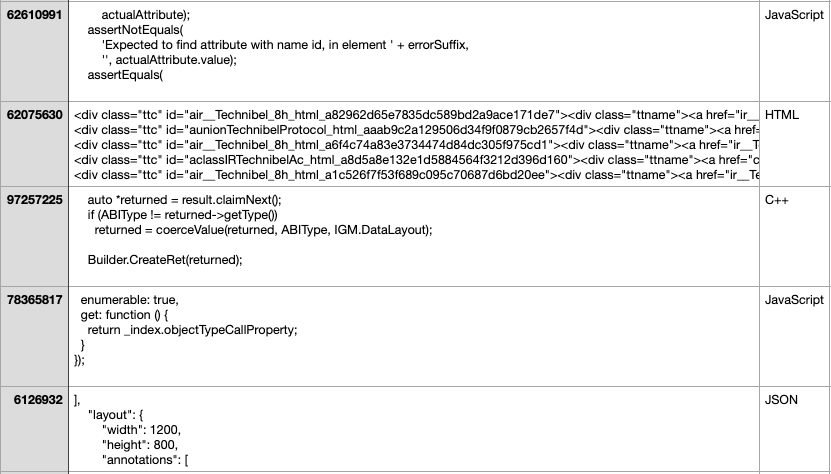
\includegraphics[width=\linewidth, height=10cm,keepaspectratio]{figures/dataset4.png}
  \caption{The processed dataset}
\end{figure}

\newpage
The quantity of each programming language is shown in Figure 6.6. 
\begin{figure}[ht]
	\centering
	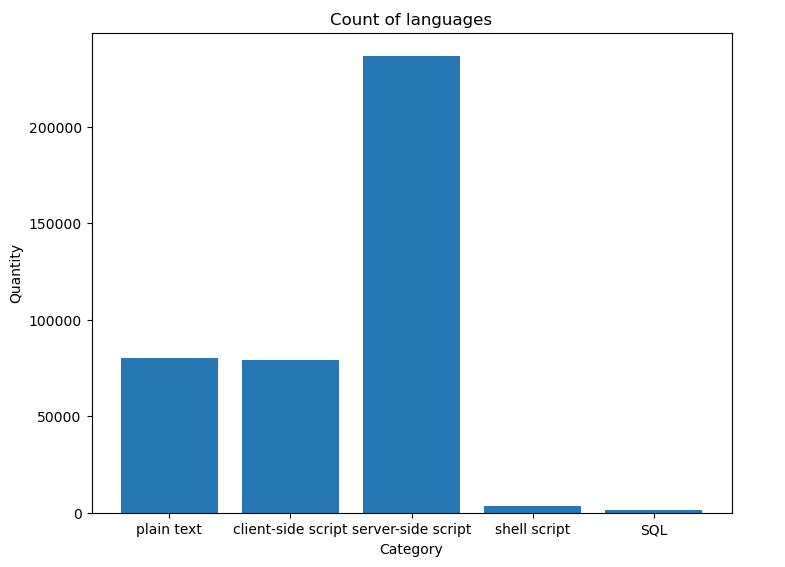
\includegraphics[width=\linewidth, height=10cm,keepaspectratio]{figures/quantity of programming language.png}
  \caption{The quantity of every category in the dataset}
\end{figure}
  


  